\documentclass{beamer}
\usepackage[ngerman]{babel}
\usepackage[utf8]{inputenc}
\usepackage{amsmath}
\usepackage{amsthm}
\usepackage{siunitx}
\usepackage{graphicx}
\usepackage{pgfplots}
\sisetup{locale = DE}
% Lade Beamer Stile
\usepackage{beamerthemesplit}
\usepackage{tcolorbox}
\usetheme{Rochester}
\usecolortheme{crane}


\title{Unterrichtseinheit zur Federkraft}
\subtitle{Das Hook'sche\footnote{Robert Hook, engl. Physiker (1635 bis 1703)}  Gesetz}
\author{Heiko Schröter}
\date{\today}

\setbeamertemplate{enumerate item}{\alph{enumi})}

\begin{document}

\frame{\titlepage}

\frame
{
  \frametitle{Federkraft}
  Kräfte sind die Ursachen für die Verformung von Körpern, z.B. für die Dehnung eines Gummibandes bzw. einer Feder oder für die Biegung eines Stahlträgers.
    \begin{figure}
	  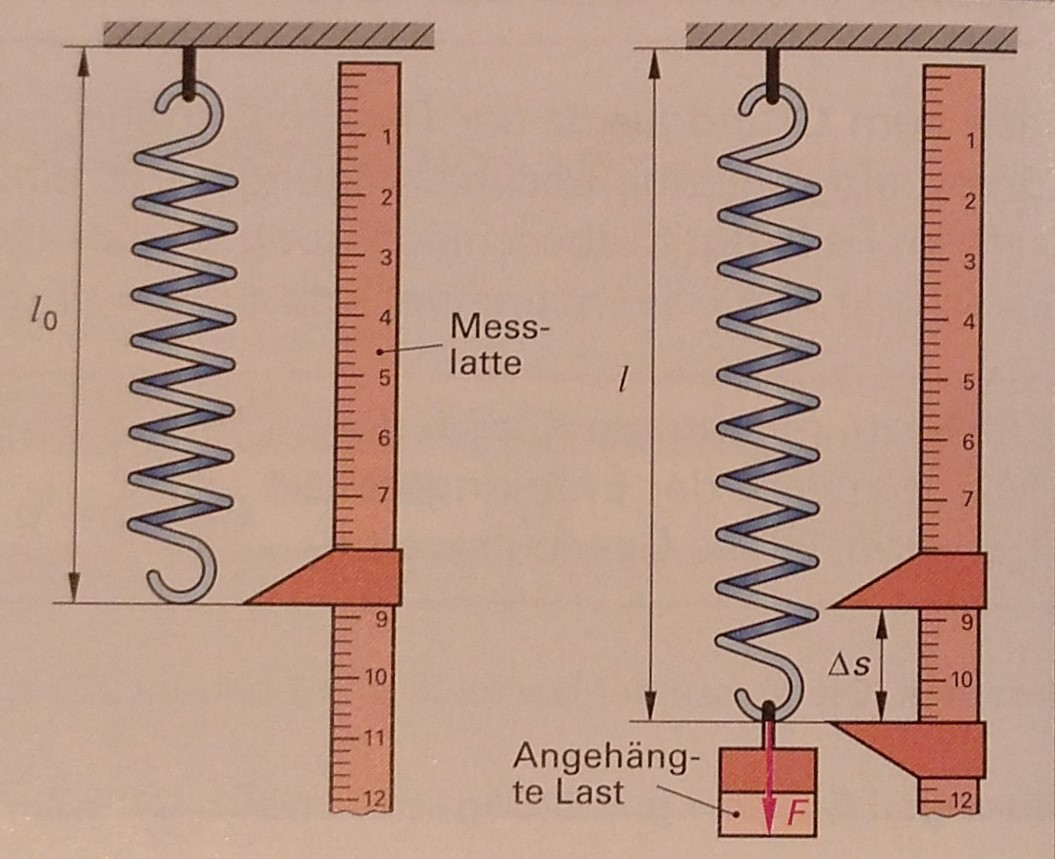
\includegraphics[width=0.5\textwidth]{Federkraft.jpg}
	  \vspace{-3mm}
	  \caption{Elastische Dehnung einer Schraubenfeder}
   \end{figure}  
}

\frame
{
  \frametitle{Ziele für die heutige Unterrichtseinheit}
  \textbf{Das Gesetz von Hooke}
  \begin{itemize}
	\item Wie verändert sich die Länge einer Feder bei Einwirkung einer Kraft?
	\item Wie ist ein Federkraftmesser aufgebaut?
	\item Welche weiteren Möglichkeiten zur Kraftmessung gibt es?
	\item Berechnung der Änderung der Bodenfreiheit beim beladen eines LKW.
	\item Wo liegen die Grenzen zur Anwendung vom Hook'schen Gesetz?
  \end{itemize}
}

\frame[allowframebreaks]
{
  \frametitle{Versuch: Elastische Dehnung einer Schraubenfeder}
\begin{tabular}{|c|c|c|}
\hline 
\multicolumn{3}{|c|}{Messwertetabelle von Versuch 1} \\ 
\hline 
%
\hline 
$F$ in $N$ & $\Delta s$ in $\si{\meter}$ & Berechnet: $\frac{F}{\Delta s}$ in $\si{\frac{\newton}{\meter}}$ \\
\hline 
0,10 & 0,033 & 3,03 \\ 
\hline 
0,20 & 0,067 & 2,98 \\ 
\hline 
0,30 & 0,101 & 2,97 \\ 
\hline 
0,40 & 0,134 & 2,99 \\ 
\hline 
0,60 & 0,199 & 3,02 \\ 
\hline 
0,80 & 0,267 & 3,00 \\ 
\hline 
1,00 & 0,330 & 3,03 \\ 
\hline 
\end{tabular} 
}

\frame
{
  \frametitle{Versuch: Elastische Dehnung einer Schraubenfeder}
  \begin{tikzpicture}
    \begin{axis}[
	%axis x line=center,
	height=6cm,
	width=\textwidth,
	compat=newest,
	title=Kraft-Verlängerungs-Diagramm,
	xlabel=Verlängerung $\Delta s$,
	ylabel=Kraft $F$,
	xmin=0, xmax=0.35,
	ymin=0, ymax=1.2,
	xticklabel style={
		/pgf/number format/fixed,
		/pgf/number format/precision=3,
		rotate=-30
		},
	xtick={0.033,0.067,0.101,0.134,0.199,0.267,0.330},
 	enlargelimits=false,
    grid = major,
]
	\addplot [color=red, thin, mark=x, domain=0:0.3] coordinates {
	(0,0)
    (0.033,0.10)
    (0.067,0.20)
    (0.101,0.30)
    (0.134,0.40)
    (0.199,0.60)
    (0.267,0.80)
    (0.330,1.00)
	};
	%\draw[help lines, dashed] {(axis cs:0.033,0) -- (axis cs:0.033,0.1)
	%(axis cs:0.067,0) -- (axis cs:0.067,0.2)};
	%\coordinate (A) at ({axis cs:0.033,0});
    %\coordinate (B) at ({axis cs:0.067,0});
   \end{axis}
   %\node[pin={below:0.033}] at (A) {};
   %\node[pin={below:0.067}] at (B) {};
  \end{tikzpicture}
}

\frame
{
  \frametitle{Das Gesetz von Hooke}
  \begin{theorem}[Die elastische Verlängerung eines Körpers ist der wirkenden Kraft proportional]
  $F=c\cdot s \Rightarrow c=\dfrac{F}{s}$
  \end{theorem}
  Dabei ist:
  \begin{description}
  \item $F=$ Federkraft in N
  \item $s=$ Federweg in mm
  \item $c=$ Federsteifigkeit (Federkonstante)
  \end{description}
  \begin{tabular}{c|c|c}
  $c$ & $F$ & $s$ \\ 
  \hline 
  $\frac{N}{mm}$ & $N$ & $mm$ \\ 
  \end{tabular} 
}

\frame{
\frametitle{Aufbau eines Federkraftmessers}
\begin{small}
\textbf{Federkraftmesser} bestehen aus zwei ineinander geschobenen Hülsen, die über eine Schraubenfeder verbunden sind. Hängt man eine Last an, so wird die Feder gedehnt und die innere Hülse herausgezogen. Sie enthält eine Skalierung, an der die Kraft abgelesen werden kann. Wegen des proportionalen Zusammenhangs zwischen Federkraft $F$ und der Verlängerung $\Delta s$ (Hooke’sches Gesetz) ist die Skala linear.
\end{small}
    \begin{figure}
	  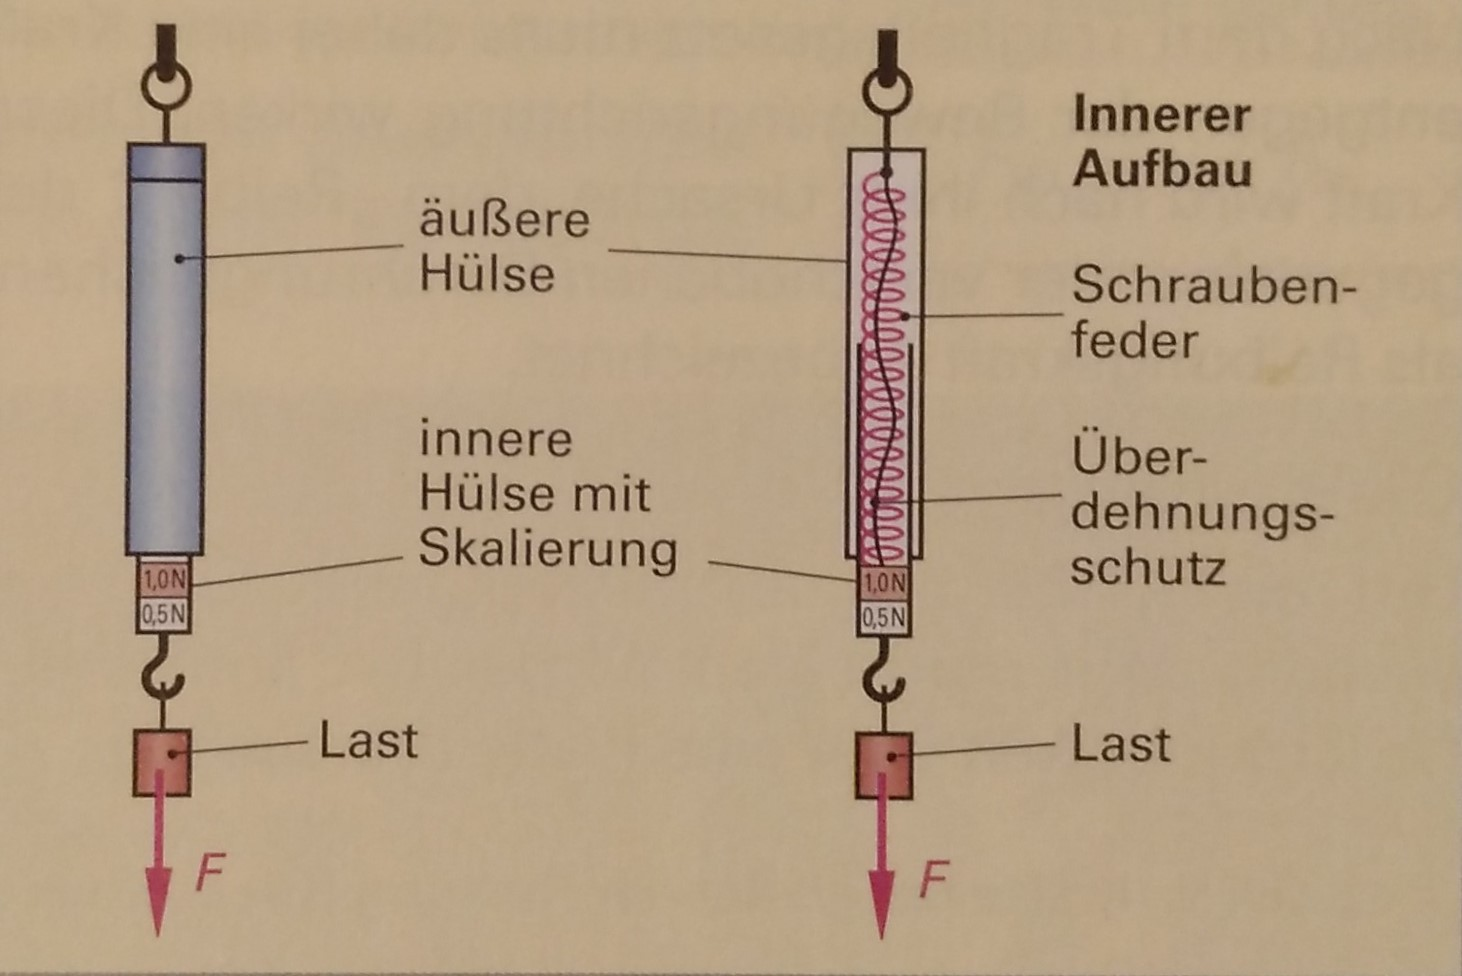
\includegraphics[width=0.45\textwidth]{Federkraftmesser.jpg}
	  \vspace{-3mm}
	  \caption{Federkraftmesser}
   \end{figure}
}

\frame{
\frametitle{Übersicht über den Aufbau von Kraftmessern}
    \begin{figure}
	  \includegraphics[width=0.8\textwidth]{methoden.jpg}
	  \vspace{-3mm}
	  \caption{Methoden der Kraftmessung}
   \end{figure}
}

\frame{
\frametitle{Beispielaufgabe 1}
\uncover<1->
{
\textbf{Aufgabe:}\\
Die Bodenfreiheit eines Lkw verringert sich bei Beladung mit einer Last von $\SI{1.5}{\tonne}$ um $\SI{50}{\milli\meter}$. Berechnen Sie die Federkonstante der gesamten Federung.\\

}
\uncover<2->
{
\vspace{1cm}
\textbf{Lösung:}\\
\begin{align*}
c=\dfrac{F}{\Delta s}=\dfrac{m\cdot g}{\Delta s}\approx\dfrac{\SI{1.5}{\tonne}\cdot \SI{10}{\frac{\newton}{\kilogram}}}{\SI{50}{\milli\meter}}=\dfrac{\SI{1500}{\kilogram}\cdot \SI{10}{\frac{\newton}{\kilogram}}}{\SI{0.050}{\meter}}=\SI{300000}{\frac{\newton}{\meter}}
\end{align*}
}
}
\end{document}
